%%----------------------------------------------------------------------------
%% Presentatie HoGent Bedrijf en Organisatie
%%----------------------------------------------------------------------------
%% Auteur: Bert Van Vreckem [bert.vanvreckem@hogent.be]

\documentclass{beamer}

%==============================================================================
% Aanloop
%==============================================================================

%---------- Packages ----------------------------------------------------------

\usepackage{graphicx,multicol}
\usepackage{comment,enumerate,hyperref}
\usepackage{amsmath,amsfonts,amssymb}
\usepackage{tikz}
\usepackage[dutch]{babel}
\usepackage[utf8]{inputenc}
\usepackage{multirow}
\usepackage{eurosym}
\usepackage{listings}
\usepackage[T1]{fontenc}
\usepackage{lmodern}
\usepackage{textcomp}
\usepackage{framed}
\usepackage{wrapfig}

%---------- Configuratie ------------------------------------------------------

\usetikzlibrary{arrows,shapes,backgrounds,positioning,shadows}

\usetheme{hogent}

%---------- Commando-definities -----------------------------------------------

\newcommand{\tabitem}{~~\llap{\textbullet}~~}

%---------- Info over de presentatie ------------------------------------------

\title[Intro]{OZT voor docenten}
\author{Jens Buysse, Bert {Van Vreckem}}
\date{AJ 2017-2018}

\newcommand{\voorstelSemEen}{29/09/2017}
\newcommand{\feedbackVoorstelSemEen}{06/10/2017}
\newcommand{\indienenBPSemEen}{08/01/2018}

\newcommand{\voorstelSemTwee}{11/12/2017}
\newcommand{\feedbackVoorstelSemTwee}{22/12/2017}
\newcommand{\indienenBPSemTwee}{28/05/2018}

\newcommand{\indienenBPderdeeEx}{20/08/2018}

%==============================================================================
% Inhoud presentatie
%==============================================================================

\begin{document}
% Data inladen 2017 - 2018

%---------- Front matter ------------------------------------------------------

% Dia met het HoGent logo
\HoGentLogo

% Titeldia met faculteitslogo
\titleframe

%---------- Inhoud ------------------------------------------------------------

\begin{frame}
  \frametitle{Inhoud}

  \tableofcontents
\end{frame}

\section{Wat is de Bachelorproef - ECTS}

\begin{frame}{}
	
	\begin{alertblock}{Eindcompetenties}
			De student kan bestaande en innovatieve (IT-)oplossingen op een methodologisch correcte manier kritisch onderzoeken, evalueren en (her)ontwerpen of optimaliseren
	\end{alertblock}

\end{frame}

\begin{frame}{Doelstellingen}
	\begin{enumerate}
		\item Kan een \textcolor{HoGentAccent1}{concrete doelstelling} en onderzoeksvragen voor een eigen onderzoeksonderwerp formuleren en verduidelijken 
		\item Kan de data \textcolor{HoGentAccent1}{methodologisch verantwoord} verzamelen 
		\item Kan \textcolor{HoGentAccent1}{methodologisch verantwoorde} analyses maken van de verzamelde data 
		\item Kan de onderzoeksvraag onderbouwd beantwoorden a.d.h.v. correcte methodologische analyses van de verzamelde data en door \textcolor{HoGentAccent1}{verschillende alternatieve oplossingen} te evalueren 
		\item Kan in functie van de onderzoeksvragen \textcolor{HoGentAccent1}{geschikte vakliteratuur} evalueren, selecteren en verwerken in een literatuurstudie 
		\item Kan een \textcolor{HoGentAccent1}{gestructureerd wetenschappelijk document} schrijven, voorzien van \textcolor{HoGentAccent1}{referenties} en conform de aangereikte template
	\end{enumerate}
\end{frame}

\begin{frame}{Doelstellingen}
	In deze sessie gaan we na welke tools ze tot hun beschikking hebben en  welke kennis ze vergaard hebben gedurende hun traject.
\end{frame}


\section{Verloop Bachelorproef 2017-2018}

\begin{frame}{Verloop BP 2017- 2018}
	\begin{enumerate}
		\item Je zoekt een onderwerp en een co-promotor
		\item Je schrijft een bachelorproefvoorstel volgens de richtlijnen
		\item Je dient het voorstel in
		\begin{itemize}
			\item semester 1 : \textcolor{HoGentAccent1}{\voorstelSemEen{}}
			\item semester 2 : \textcolor{HoGentAccent1}{\voorstelSemTwee{}}
		\end{itemize}
		\item  Je krijgt feedback op uw voorstel
		\begin{itemize}
			\item semester 1: \textcolor{HoGentAccent1}{\feedbackVoorstelSemEen{}}
			\item semester 2: \textcolor{HoGentAccent1}{\feedbackVoorstelSemTwee{}}
		\end{itemize} 
		\item Je maakt de bachelorproef volgens de richtlijnen
		\item Je dient uw bachelorproef in volgens de richtlijnen
		\begin{itemize}
			\item semester 1: \textcolor{HoGentAccent1}{\indienenBPSemEen{}}
			\item semester 2: \textcolor{HoGentAccent1}{\indienenBPSemTwee{}}
			\item herexamen: \textcolor{HoGentAccent1}{\indienenBPderdeeEx{}}
		\end{itemize}
		\item Je verdedigt uw BP voor een jury 
	\end{enumerate}
\end{frame}



\section{Kan een concrete doelstelling en onderzoeksvragen voor een eigen onderzoeksonderwerp formuleren en verduidelijken}

\sectionframelogo{}

\subsection{Een BP-onderwerp}
\begin{frame}{Een onderwerp kiezen}
	
	\begin{columns}[c]

		\column{.5\textwidth}

		\begin{itemize}
			\item \textcolor{HoGentAccent3}{ICT-gerelateerd onderwerp
			\item Voldoende uitdagend, maar realistisch
			\item Concreet probleem/vraag uit het werkveld
			\item Gaat verder dan het verzamelen van informatie
			\item Nuttig voor anderen in je vakgebied
			\item Origineel en individueel (Een BP met twee gaat niet)}
		\end{itemize}
	
	
	
		\column{.5\textwidth}

	\begin{itemize}
		\item \textcolor{HoGentAccent2}{Zuivere literatuurstudie
		\item Programmeerproject
		\item Vergelijking van frameworks, producten, services zonder
		concrete case, zonder requirementsanalyse
		\item  Hergebruik resultaten stage}
	\end{itemize}
		
	\end{columns}	
	
\end{frame}


\begin{frame}{Tools tot het vinden van een onderwerp}
	\begin{enumerate}
		\item In OZT maken ze reeds een BP onderwerp
		\item De BP-gids bevat veel tips rond het zoeken naar een onderwerp
		\item Er zijn externe voorstellen op het forum van Chamilo van bedrijven
		\item \textcolor{HoGentAccent1}{Externe voorstellen van de docenten}
	\end{enumerate}
\end{frame}

\section{Kan de data methodologisch verantwoord verzamelen}
\sectionframelogo{}
\subsection{De Wetenschappelijke methode}

\begin{frame}
  \scaledimg{img/les1-01}
\end{frame}


\begin{frame}
  \frametitle{De wetenschappelijke methode}

  Aan de hand van \textbf{empirisch onderzoek} zijn we geïnteresseerd in volgende zaken:

  \begin{enumerate}
    \item Exploratie
    \item Beschrijving
    \item Voorspelling
    \item Controle
  \end{enumerate}
\end{frame}

\begin{frame}
  \frametitle{De wetenschappelijke methode}
    \begin{itemize}
      \item Generalisatie
        \begin{itemize}
          \item Bv. ``De LAMP stack heeft een algemeen snellere uitvoeringstijd dan een WAMP stack''
        \end{itemize}
      \item Verstaan, begrijpen
        \begin{itemize}
          \item De WAMP stack voegt een extra delay toe aan de uitvoeringstijd door het gebruik van Windows 
          \item Theorieontwikkeling
        \end{itemize}
    \end{itemize}
\end{frame}

\begin{frame}
  \frametitle{Het onderzoeksproces}

  \begin{columns}
  \column{\dimexpr\paperwidth}
  \begin{center}
    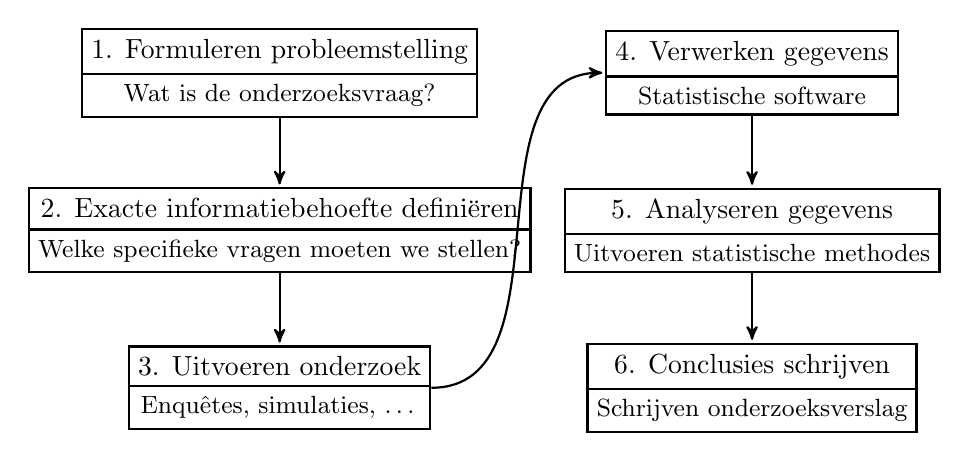
\begin{tikzpicture}[
      auto,
      thick,
      ->,
      >=stealth',
      shorten >=1pt,
      node distance=2cm,
      fase/.style={
        shape=rectangle split,
        rectangle split parts=2,
        ,
        draw}]


      \node[fase] (1) {
        1. Formuleren probleemstelling
        \nodepart{second}
        \small{Wat is de onderzoeksvraag?}
      };
      \uncover<2->{\node[fase] (2) [below of=1] {
        2. Exacte informatiebehoefte definiëren
        \nodepart{second}
        \small{Welke specifieke vragen moeten we stellen?}
      };}
      \uncover<3->{\node[fase] (3) [below of=2] {
        3. Uitvoeren onderzoek
        \nodepart{second}
        \small{Enquêtes, simulaties, \ldots}
      };}
      \uncover<4->{\node[fase] (4) [right of=1, node distance=6cm] {
        4. Verwerken gegevens
        \nodepart{second}
        \small{Statistische software}
      };}
      \uncover<5->{\node[fase] (5) [below of=4] {
        5. Analyseren gegevens
        \nodepart{second}
        \small{Uitvoeren statistische methodes}
      };}
      \uncover<6->{\node[fase] (6) [below of=5] {
        6. Conclusies schrijven
        \nodepart{second}
        \small{Schrijven onderzoeksverslag}
      };}

      \uncover<2->{\draw (1) -- (2);}
      \uncover<3->{\draw (2) -- (3);}
      \uncover<4->{\draw (3.east) to [out=0,in=180] (4.west);}
      \uncover<5->{\draw (4) -- (5);}
      \uncover<6->{\draw (5) -- (6);}
    \end{tikzpicture}
  \end{center}
\end{columns}

\end{frame}


\begin{frame}
  \frametitle{Meetniveaus}

  Kwalitatieve schalen:

  \begin{description}
    \item[Nominaal] Categorieën. Bv. Geslacht, ras, land, vorm, \ldots
    \item[Ordinaal] Volgorde. Bv. militaire rang, opleidingsniveau, \ldots
  \end{description}

\end{frame}

\begin{frame}
  \frametitle{Meetniveaus}

  Kwantitatieve schalen:

  \begin{description}
    \item[Interval] Meting: getal + meeteenheid, nulpunt niet belangrijk\\
      bv. 20°C - 15°C = 5°C, maar 20°C is \emph{NIET} 1/3 warmer dan 15°C
    \item[Ratio] Meting t.o.v. absoluut nulpunt. bv. Afstand (m), energie (J), massa (kg), \ldots\\
      bv. 20m is \emph{wel} 1/3 langer dan 15m
  \end{description}
\end{frame}



\end{document}
